\section{Geometry Generation}

Designing a good model geometry is critical as it can save significant computational resources.
When designing a geometry the FEM user should try to represent the model geometry as accurately as possible while:
\begin{enumerate}
  \item Avoid unnecessarily fine details; these may require an excessively fine mesh to resolve.
  \item Leverage symmetry to reduce geometry size and thereby the mesh.
\end{enumerate}\par
Achieving these goals is not always straightforward, and depend on the skill of the modeler and on the available tools.
Typically a model geometry is constructed in some computer assisted design (CAD) software, and the particular tools available in these vary by software.\par

COMSOL has a built-in geometry generation tool, which allows the construction of advanced geometries by performing various operations on simpler geometries, e.g. a cylinder and half sphere can be combined to make a rivet.
It is also possible to import pre-generated geometries from other CAD software.
However, we will create our own geometry.\par

The interior, or indeed the house itself will not be explicitly modeled, instead we will only consider the soil surrounding the house.
This is done for the simple reason that interiors are simply too heterogenous to generalize in any meaningful way.
Even if the interior was explicitly modeled, it would be prohibitively expensive to do, as it would require solving the Navier-Stokes equation.
Instead the interior is implicitly modeled as a CSTR and simply coupled with the explicit geometry via the foundation crack boundary.\par

One of the nice properties of our VI scenario is that, due to symmetry, we only need to explicitly model a quarter of it.
This reduces the number of required mesh points by 75\%, which is a huge computational saving.
To create our quarter geometry, only a few simple geometric objects and Boolean operations are required: two cuboids, two rectangles, one Boolean difference operation, and one Boolean join operation.
Figure \ref{fig:geometry} shows the resulting geometry.
Note that $z = \SI{0}{\metre}$ is the groundwater/soil interface and the plane of symmetry is around the $(x, y) = (\SI{0}{\metre},\SI{0}{\metre})$ axis\par

To create the soil surrounding the building:
\begin{enumerate}
  \item Create a \SI{15}{\metre} by \SI{15}{\metre} by \SI{4}{\metre} block with its base at $(x, y, z) = (\SI{0}{\metre},\SI{0}{\metre},\SI{0}{\metre})$. This is the entire soil domain.
  \item Create a \SI{5}{\metre} by \SI{5}{\metre} by \SI{1}{\metre} block with its base at $(x, y, z) = (\SI{0}{\metre},\SI{0}{\metre},\SI{3}{\metre})$. This will represent the volume that the house take up in the soil, i.e. the underground portion of the basement.
  \item Perform a difference operation, removing the "basement" block from the "soil" block.
\end{enumerate}
At this point you will see that a quarter soil domain has been created, with an empty space that represents a house with a foundation slab located \SI{1}{\metre} bgs.\par

The foundation crack will be modeled by joining two  \SI{1}{\centi\metre} wide strip that spans the perimeter of the surface that represents the house foundation.
This strip is created by joining two rectangles on foundation surface:
\begin{enumerate}
  \item Define a work plane \SI{3}{\metre} above zero. This allows us to place two-dimensional objects on the surface of or inside a three-dimensional object.
  \item On the work plane create a \SI{5}{\metre} by \SI{1}{\centi\metre} rectangle with its base at $(x, y) = (\SI{0}{\metre},\SI{5}{\metre} - \SI{1}{\centi\metre})$. This represents one side of the perimeter crack.
  \item Copy the rectangle and rotate it \SI{90}{\degree} around the corner of the foundation, i.e. $(x, y) = (\SI{5}{\metre} - \SI{0.5}{\centi\metre},\SI{5}{\metre} - \SI{0.5}{\centi\metre})$.
  \item Join the two rectangles to create a unified perimeter foundation crack.
\end{enumerate}
Now the geometry of this VI scenario is complete.\par

\begin{figure}[htb!]
  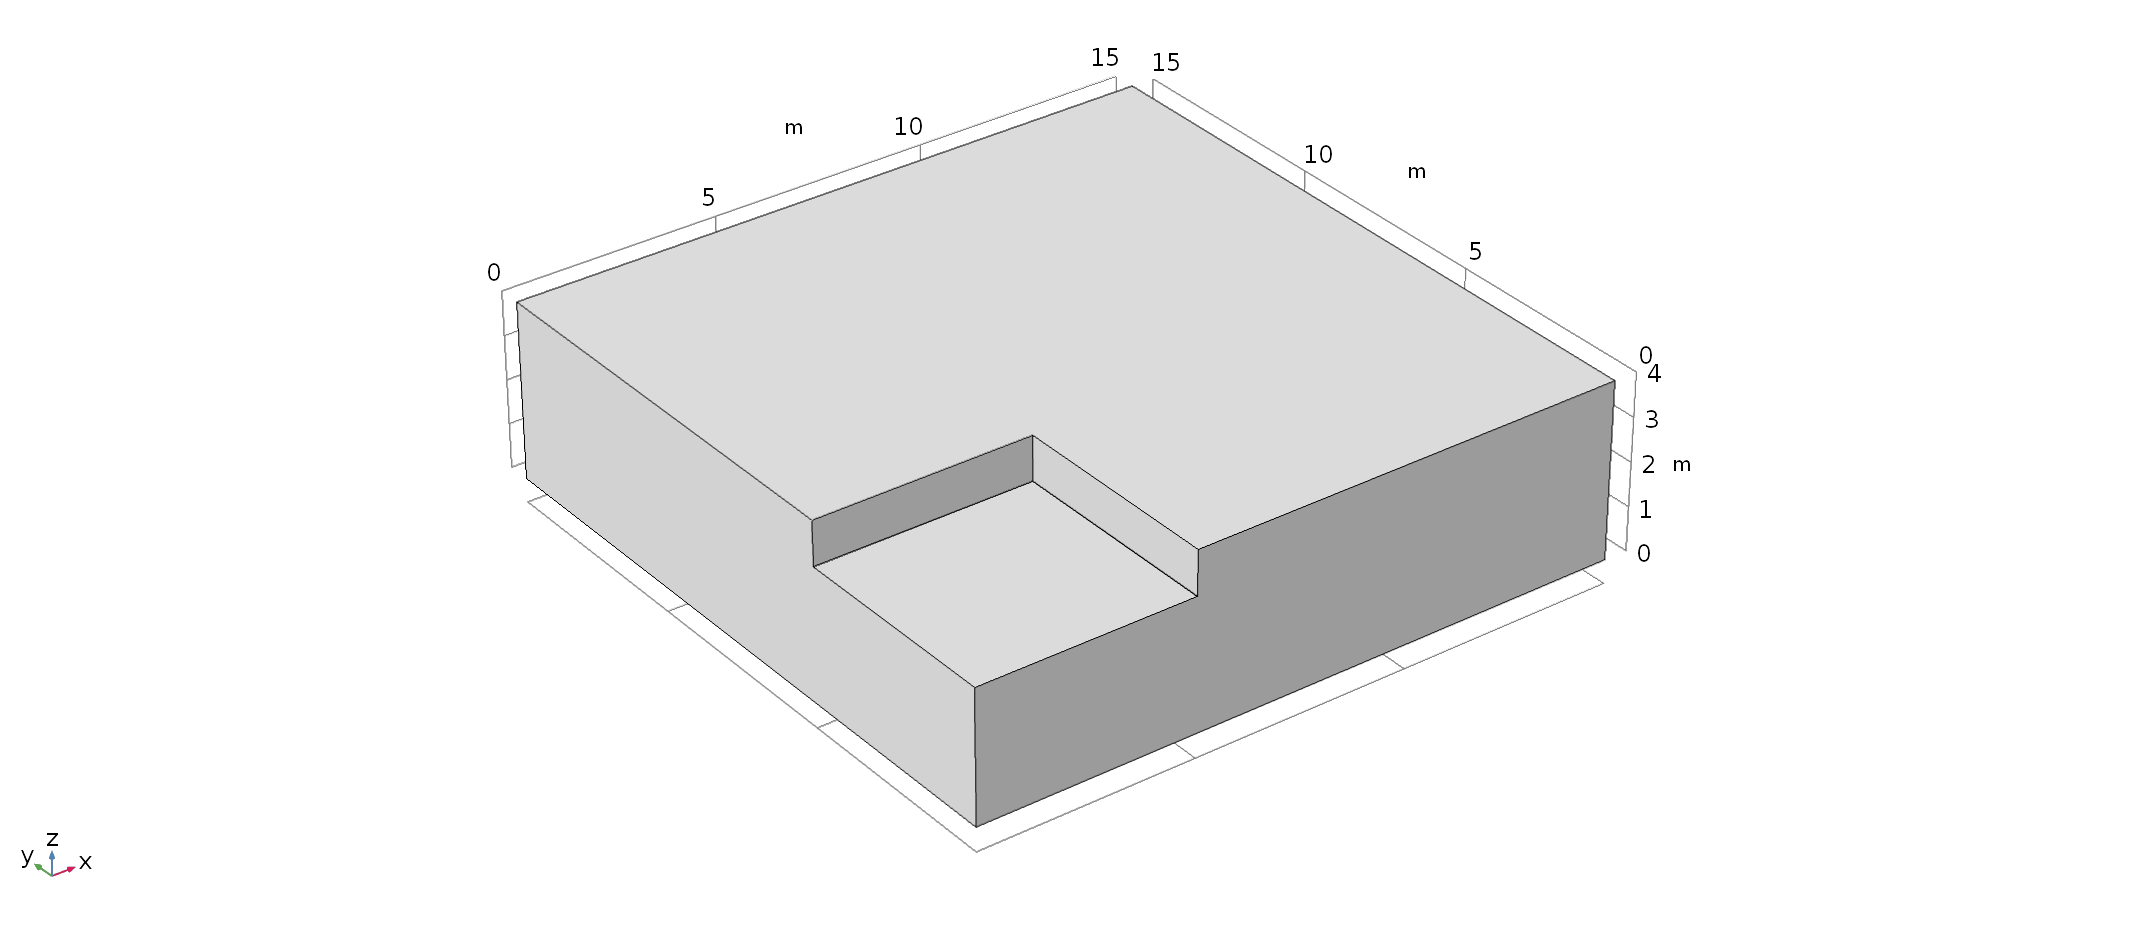
\includegraphics[width=\textwidth]{vi_model.png}
  \caption{The complete geometry of the VI scenario.}
  \label{fig:geometry}
\end{figure}
